\documentclass[12pt]{article}
\usepackage[utf8]{inputenc}
\usepackage[romanian]{babel}
\usepackage{graphicx}
\usepackage{csvsimple}
\usepackage{pdfpages}

%%%%%%%%%%%%%%%%%%%%%%%%%%%%%%%%%%%%%%%%%
% Lachaise Assignment
% Structure Specification File
% Version 1.0 (26/6/2018)
%
% This template originates from:
% http://www.LaTeXTemplates.com
%
% Authors:
% Marion Lachaise & François Févotte
% Vel (vel@LaTeXTemplates.com)
%
% License:
% CC BY-NC-SA 3.0 (http://creativecommons.org/licenses/by-nc-sa/3.0/)
% 
%%%%%%%%%%%%%%%%%%%%%%%%%%%%%%%%%%%%%%%%%

%----------------------------------------------------------------------------------------
%	PACKAGES AND OTHER DOCUMENT CONFIGURATIONS
%----------------------------------------------------------------------------------------

\usepackage{amsmath,amsfonts,stmaryrd,amssymb} % Math packages

\usepackage{enumerate} % Custom item numbers for enumerations

\usepackage[ruled]{algorithm2e} % Algorithms

\usepackage[framemethod=tikz]{mdframed} % Allows defining custom boxed/framed environments

\usepackage{listings} % File listings, with syntax highlighting
\lstset{
	basicstyle=\ttfamily, % Typeset listings in monospace font
}

%----------------------------------------------------------------------------------------
%	DOCUMENT MARGINS
%----------------------------------------------------------------------------------------

\usepackage{geometry} % Required for adjusting page dimensions and margins

\geometry{
	paper=a4paper, % Paper size, change to letterpaper for US letter size
	top=2.5cm, % Top margin
	bottom=3cm, % Bottom margin
	left=2.5cm, % Left margin
	right=2.5cm, % Right margin
	headheight=14pt, % Header height
	footskip=1.5cm, % Space from the bottom margin to the baseline of the footer
	headsep=1.2cm, % Space from the top margin to the baseline of the header
	%showframe, % Uncomment to show how the type block is set on the page
}

%----------------------------------------------------------------------------------------
%	FONTS
%----------------------------------------------------------------------------------------

\usepackage[utf8]{inputenc} % Required for inputting international characters
\usepackage[T1]{fontenc} % Output font encoding for international characters


%----------------------------------------------------------------------------------------
%	COMMAND LINE ENVIRONMENT
%----------------------------------------------------------------------------------------

% Usage:
% \begin{commandline}
%	\begin{verbatim}
%		$ ls
%		
%		Applications	Desktop	...
%	\end{verbatim}
% \end{commandline}

\mdfdefinestyle{commandline}{
	leftmargin=10pt,
	rightmargin=10pt,
	innerleftmargin=15pt,
	middlelinecolor=black!50!white,
	middlelinewidth=2pt,
	frametitlerule=false,
	backgroundcolor=black!5!white,
	frametitle={Command Line},
	frametitlefont={\normalfont\sffamily\color{white}\hspace{-1em}},
	frametitlebackgroundcolor=black!50!white,
	nobreak,
}

% Define a custom environment for command-line snapshots
\newenvironment{commandline}{
	\medskip
	\begin{mdframed}[style=commandline]
}{
	\end{mdframed}
	\medskip
}

%----------------------------------------------------------------------------------------
%	FILE CONTENTS ENVIRONMENT
%----------------------------------------------------------------------------------------

% Usage:
% \begin{file}[optional filename, defaults to "File"]
%	File contents, for example, with a listings environment
% \end{file}

\mdfdefinestyle{file}{
	innertopmargin=1.6\baselineskip,
	innerbottommargin=0.8\baselineskip,
	topline=false, bottomline=false,
	leftline=false, rightline=false,
	leftmargin=2cm,
	rightmargin=2cm,
	singleextra={%
		\draw[fill=black!10!white](P)++(0,-1.2em)rectangle(P-|O);
		\node[anchor=north west]
		at(P-|O){\ttfamily\mdfilename};
		%
		\def\l{3em}
		\draw(O-|P)++(-\l,0)--++(\l,\l)--(P)--(P-|O)--(O)--cycle;
		\draw(O-|P)++(-\l,0)--++(0,\l)--++(\l,0);
	},
	nobreak,
}

% Define a custom environment for file contents
\newenvironment{file}[1][File]{ % Set the default filename to "File"
	\medskip
	\newcommand{\mdfilename}{#1}
	\begin{mdframed}[style=file]
}{
	\end{mdframed}
	\medskip
}

%----------------------------------------------------------------------------------------
%	NUMBERED QUESTIONS ENVIRONMENT
%----------------------------------------------------------------------------------------

% Usage:
% \begin{question}[optional title]
%	Question contents
% \end{question}

\mdfdefinestyle{question}{
	innertopmargin=1.2\baselineskip,
	innerbottommargin=0.8\baselineskip,
	roundcorner=5pt,
	nobreak,
	singleextra={%
		\draw(P-|O)node[xshift=1em,anchor=west,fill=white,draw,rounded corners=5pt]{%
		Question \theQuestion\questionTitle};
	},
}

\newcounter{Question} % Stores the current question number that gets iterated with each new question

% Define a custom environment for numbered questions
\newenvironment{question}[1][\unskip]{
	\bigskip
	\stepcounter{Question}
	\newcommand{\questionTitle}{~#1}
	\begin{mdframed}[style=question]
}{
	\end{mdframed}
	\medskip
}

%----------------------------------------------------------------------------------------
%	WARNING TEXT ENVIRONMENT
%----------------------------------------------------------------------------------------

% Usage:
% \begin{warn}[optional title, defaults to "Warning:"]
%	Contents
% \end{warn}

\mdfdefinestyle{warning}{
	topline=false, bottomline=false,
	leftline=false, rightline=false,
	nobreak,
	singleextra={%
		\draw(P-|O)++(-0.5em,0)node(tmp1){};
		\draw(P-|O)++(0.5em,0)node(tmp2){};
		\fill[black,rotate around={45:(P-|O)}](tmp1)rectangle(tmp2);
		\node at(P-|O){\color{white}\scriptsize\bf !};
		\draw[very thick](P-|O)++(0,-1em)--(O);%--(O-|P);
	}
}

% Define a custom environment for warning text
\newenvironment{warn}[1][Warning:]{ % Set the default warning to "Warning:"
	\medskip
	\begin{mdframed}[style=warning]
		\noindent{\textbf{#1}}
}{
	\end{mdframed}
}

%----------------------------------------------------------------------------------------
%	INFORMATION ENVIRONMENT
%----------------------------------------------------------------------------------------

% Usage:
% \begin{info}[optional title, defaults to "Info:"]
% 	contents
% 	\end{info}

\mdfdefinestyle{info}{%
	topline=false, bottomline=false,
	leftline=false, rightline=false,
	nobreak,
	singleextra={%
		\fill[black](P-|O)circle[radius=0.4em];
		\node at(P-|O){\color{white}\scriptsize\bf i};
		\draw[very thick](P-|O)++(0,-0.8em)--(O);%--(O-|P);
	}
}

% Define a custom environment for information
\newenvironment{info}[1][Info:]{ % Set the default title to "Info:"
	\medskip
	\begin{mdframed}[style=info]
		\noindent{\textbf{#1}}
}{
	\end{mdframed}
}

% @arcilli
\renewcommand\refname{}
\lstset{frame=tb,
	language=Java,
	aboveskip=3mm,
	belowskip=3mm,
	showstringspaces=false,
	columns=flexible,
	basicstyle={\small\ttfamily},
	numbers=none,
	numberstyle=\tiny\color{gray},
	keywordstyle=\color{blue},
	commentstyle=\color{dkgreen},
	stringstyle=\color{mauve},
	breaklines=true,
	breakatwhitespace=true,
	tabsize=3
}
\usepackage{listings}
\usepackage{color}
\definecolor{dkgreen}{rgb}{0,0.6,0}
\definecolor{gray}{rgb}{0.5,0.5,0.5}
\definecolor{mauve}{rgb}{0.58,0,0.82}
\renewcommand{\contentsname}{Cuprins}
\renewcommand*{\algorithmcfname}{Algoritm}
\usepackage{graphicx}
\graphicspath{ {./images/} }
\usepackage{indentfirst} % Include the file specifying the document structure and custom commands
\title{Ingineria programării. Proiect: inferența prin enumerare} % Title of the assignment

\author{\textbf{Nicolae Boca, Ștefan Ignătescu, Gabriel Răileanu}\\ \texttt{1409A}}
\date{mai 2020}

\begin{document}

\maketitle % Print the title

\section{Introducerea}
Programul de față calculează probabilitățile de apariție ale unor afecțiuni medicale, pe baza datelor deja existente despre anumite comorbidități. Pe baza probabilităților deja cunoscute, se pot defini noduri observate și noduri evidență.
\par
Proiectul de față își propune respectarea unor standarde în ceea ce privește stilul codului, tratarea excepțiilor, dar și modalitățile în care se realizează testarea unităților.
\par
De asemenea, s-au urmărit toate etapele prezente în dezvoltarea unui produs software (proiectare, implementare, testare și livrarea artefactului software).
\section{Diagrame UML}
diagramele UML: cazuride utilizare, clase, activități, secven
\section{Modul de utilizare al programului}
Aplicația dispune de o interfață grafică din care utilizatorul poate seta valorile probabilităților pentru afecțiunile disponibile. De asemenea, există posibilitatea importării unui set predefinit de date (cele folosite în cadrul laboratorului de inteligență artificială), dar și opțiunea de a încărca datele dintr-un fișier, care trebuie să respecte un anumit format, ilustrat în tabelul \ref{probabilitiesFileFormatTable}.

\begin{table}[h!]
	\begin{center}
	\caption{Exemplu de format pentru probabilități, în cazul unui nod cu doi părinți}
	\label{probabilitiesFileFormatTable}
\begin{tabular}{c|c|c}
	\hline
	\textbf{first parent}&\textbf{second parent} &\textbf{val(P(x)=true)}
	\\ \hline
	true & true & value \\
	true & false & value \\
	false & true & value \\
	false & false & value \\
	\hline
\end{tabular}
\end{center}
\end{table}
În cazul introducerii valorilor de probabilitate în mod manual, utilizatorul va fi împiedicat să scrie date eronate, iar câmpurile alăturate se vor completa automat pentru a ușura acest proces.
\par
După alegerea valorilor pentru probabilități, utilizatorul poate alege din meniuri de tip radio sau drop-down nodurile de interes (noduri evidențe sau noduri observate).
\section{Testarea aplicației}
Pentru aplicatia dezvoltată au fost testate atât funcționarea în parametri	 a interfeței grafice, cât și logica pentru calcularea probabilităților condiționate. 
Aceste cazuri de test sunt prezentate în figura 1.
\begin{figure}[!h]
	\centering
	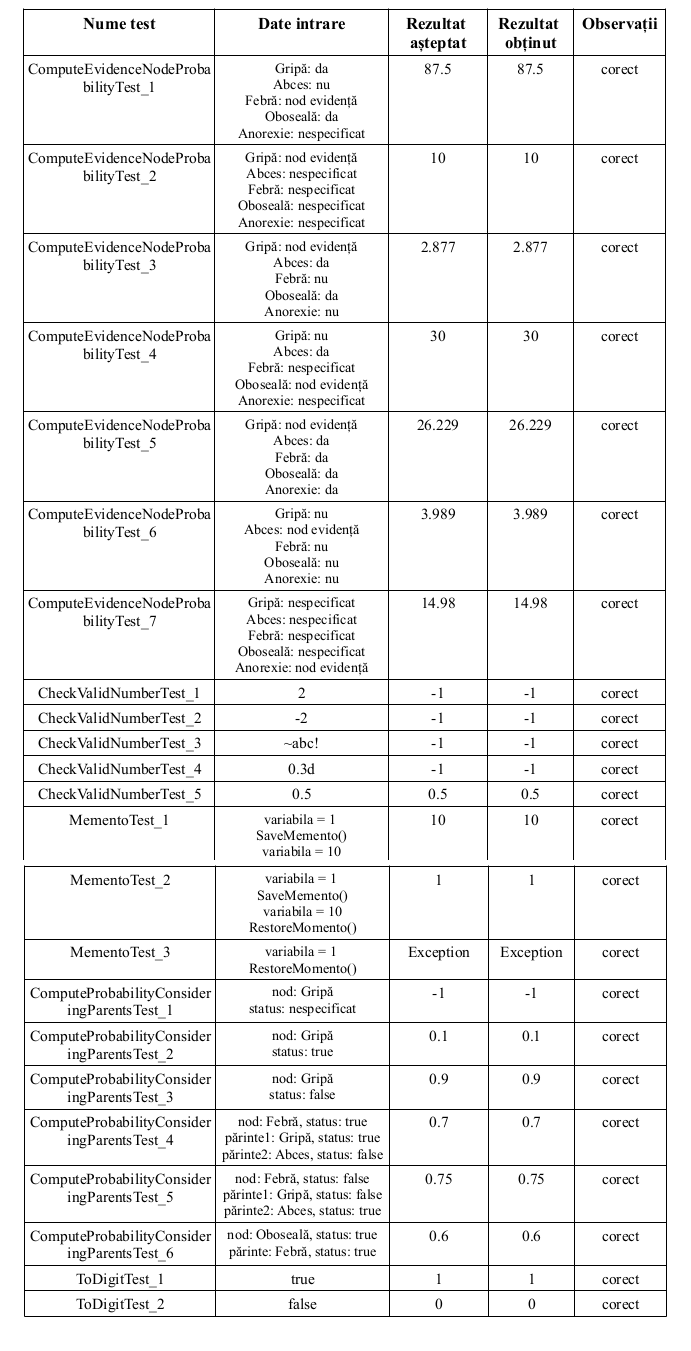
\includegraphics[scale=0.38]{raport}
	\label{fig:testCases}
	\caption{Cazurile de test}
\end{figure}
\section{Capturi de ecran}
	\begin{figure}[!h]
		\centering
		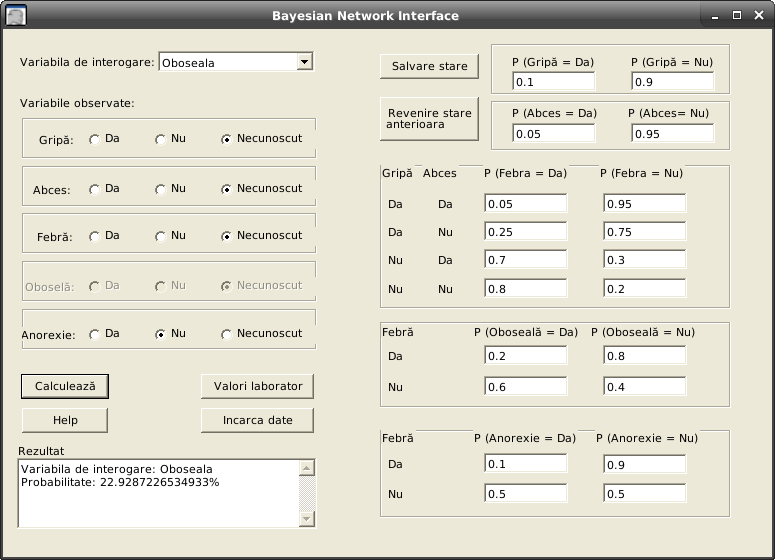
\includegraphics [scale=0.5] {img/gui.png}
		\caption{Interfața aplicației}
	\end{figure}
	\begin{figure}[!h]
	\centering
	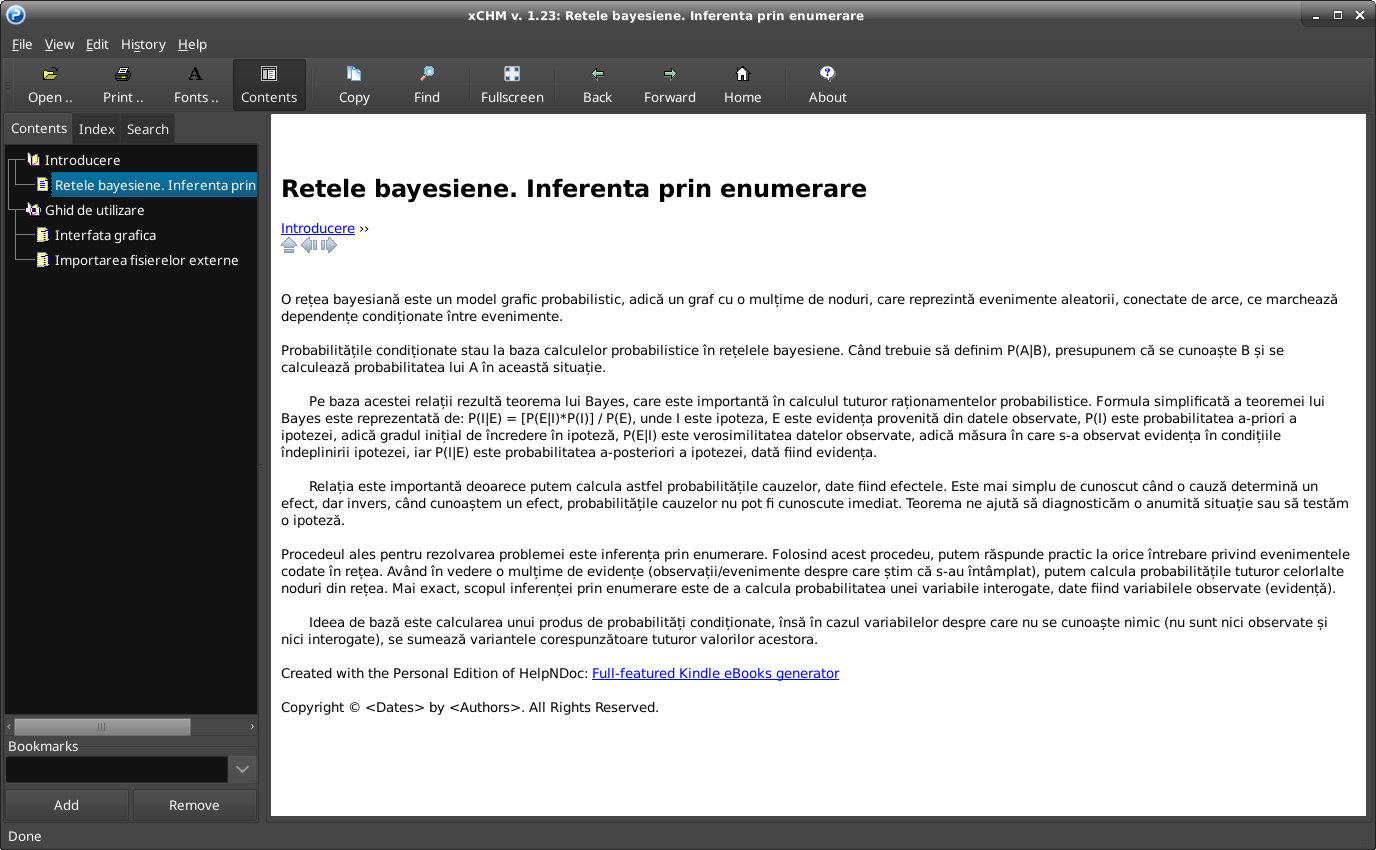
\includegraphics [scale=0.3] {img/help.png}
	\caption{Captură de ecran din meniul de \textit{help}}
\end{figure}
\section{Contribuții individuale}
\begin{itemize}
	\item \textbf{Nicolae Boca}: creare meniu \textit{help}, design cazuri de test și testarea unităților
	\item \textbf{Ștefan Ignătescu}: refactorizare, implementare șablon de proiectare, respectarea stilului de codare
	\item \textbf{Gabriel Răileanu}: documentație, document SRS, coordonare echipă
\end{itemize}
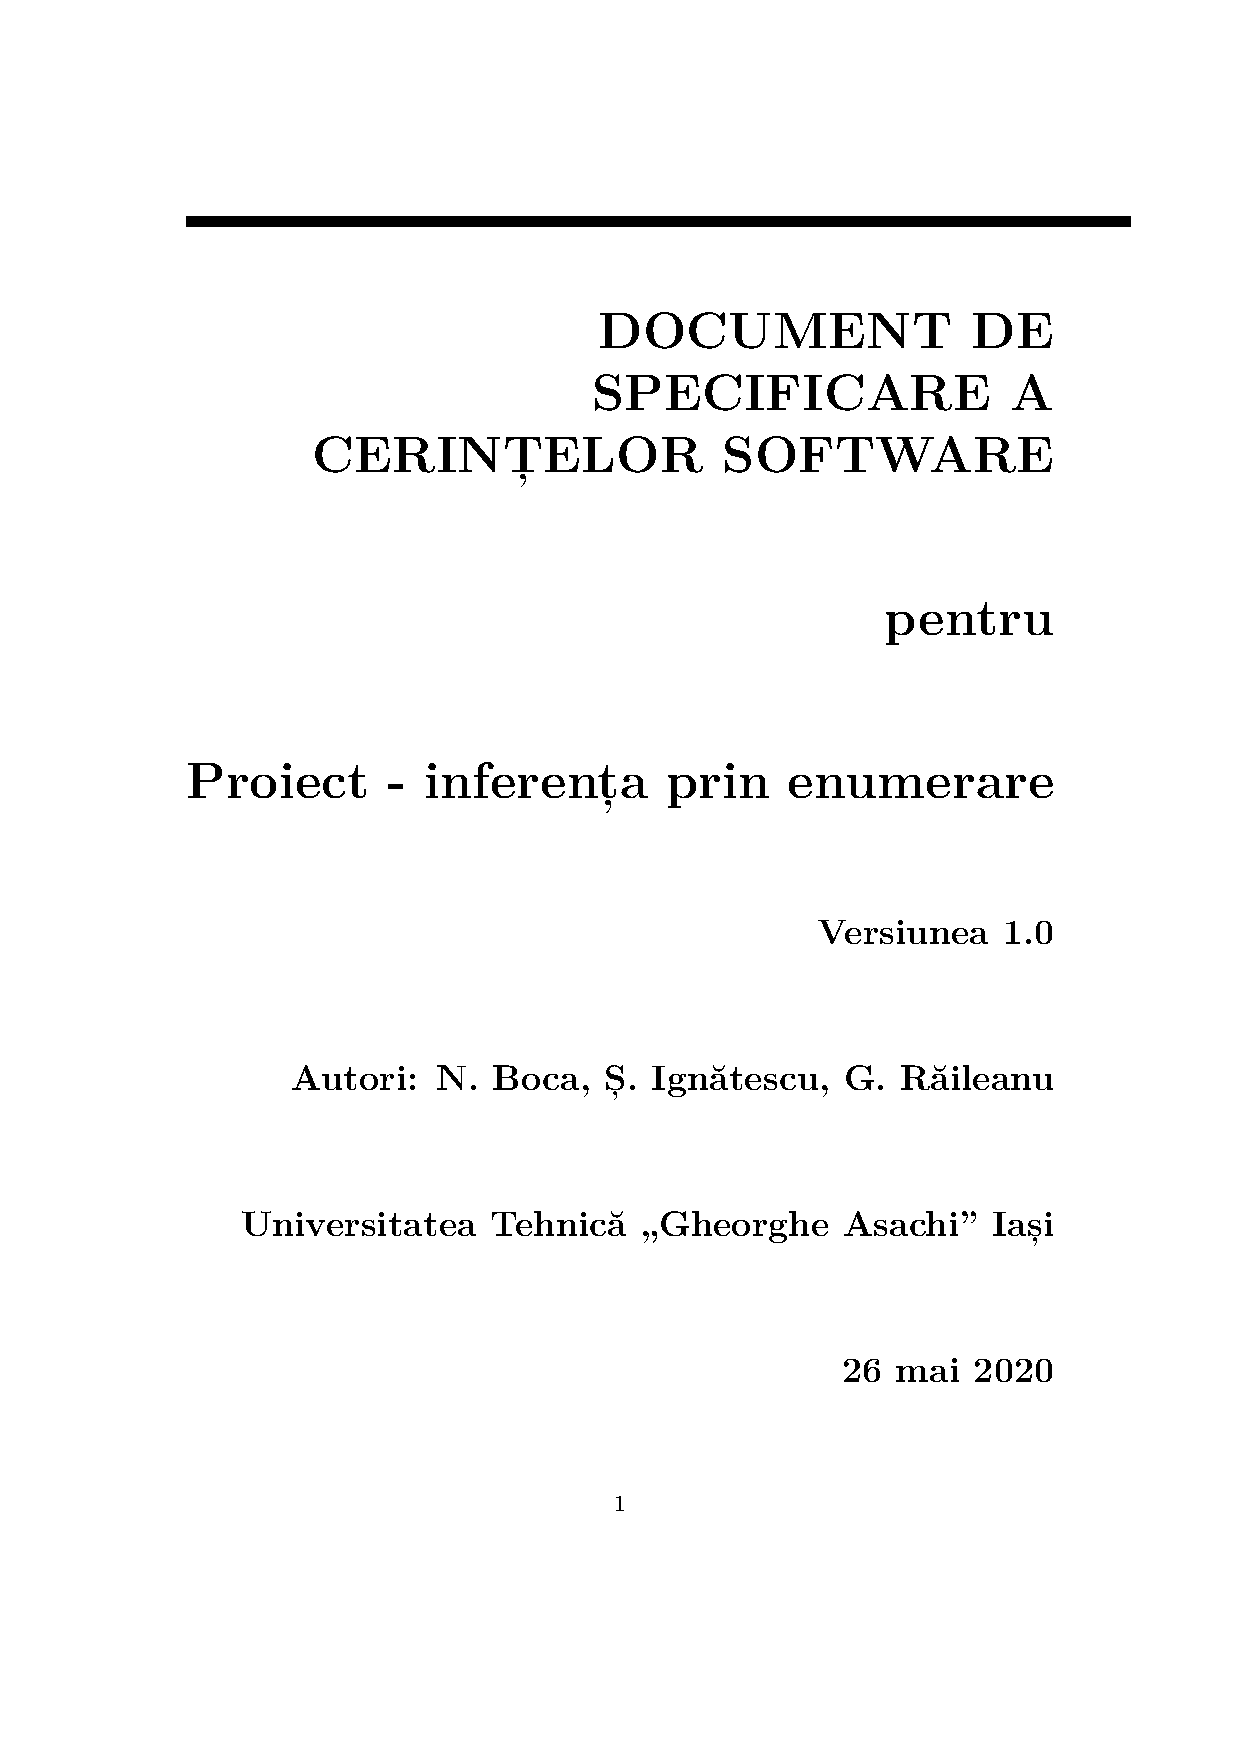
\includepdf[pages=-]{../srs/srs.pdf}
\end{document}